\section{Graphite}
\label{sec10:graphite}

\begin{itemize}
\item Outline: {\it Obtain MLWFs for the graphite (AB, Bernal).}
\end{itemize}

\begin{figure}[h!]
\centering
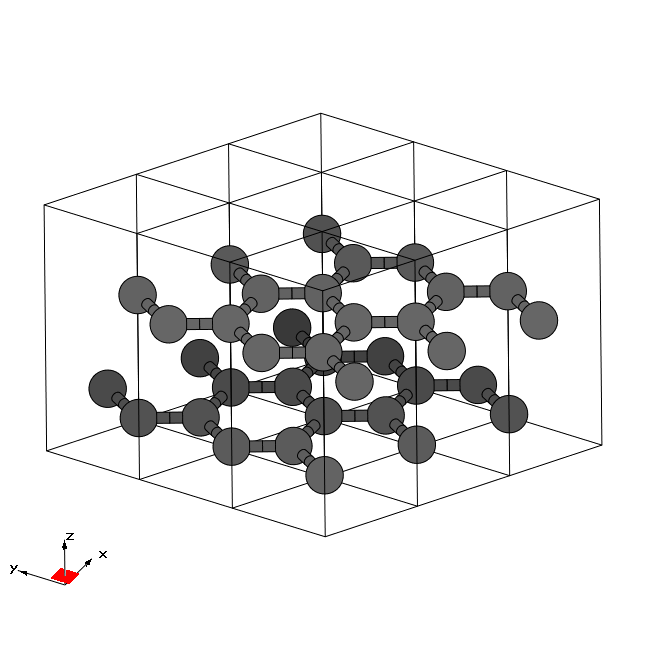
\includegraphics[width=0.25\columnwidth,trim={20pt 55pt 35pt 55pt},clip]{figure/example10/graphite.png}
\caption{Unit cell of Graphite plotted with the \xcrysden{} program.}
\label{fig10.0}
\end{figure}

\begin{itemize}
	\item[1-5] {\it Compute the MLWFs.}

	Converged values for the total spread functional and its components are shown in Tab.~\ref{tab10.1}. 
	Three MLWFs, one $\sigma$ and two $p_z$ on different layers are shown in \Fig{fig10.1}(a),(b) and (c) respectively.
\end{itemize}

\begin{figure}[h!]
\centering
\subfloat[$\sigma$ top layer]{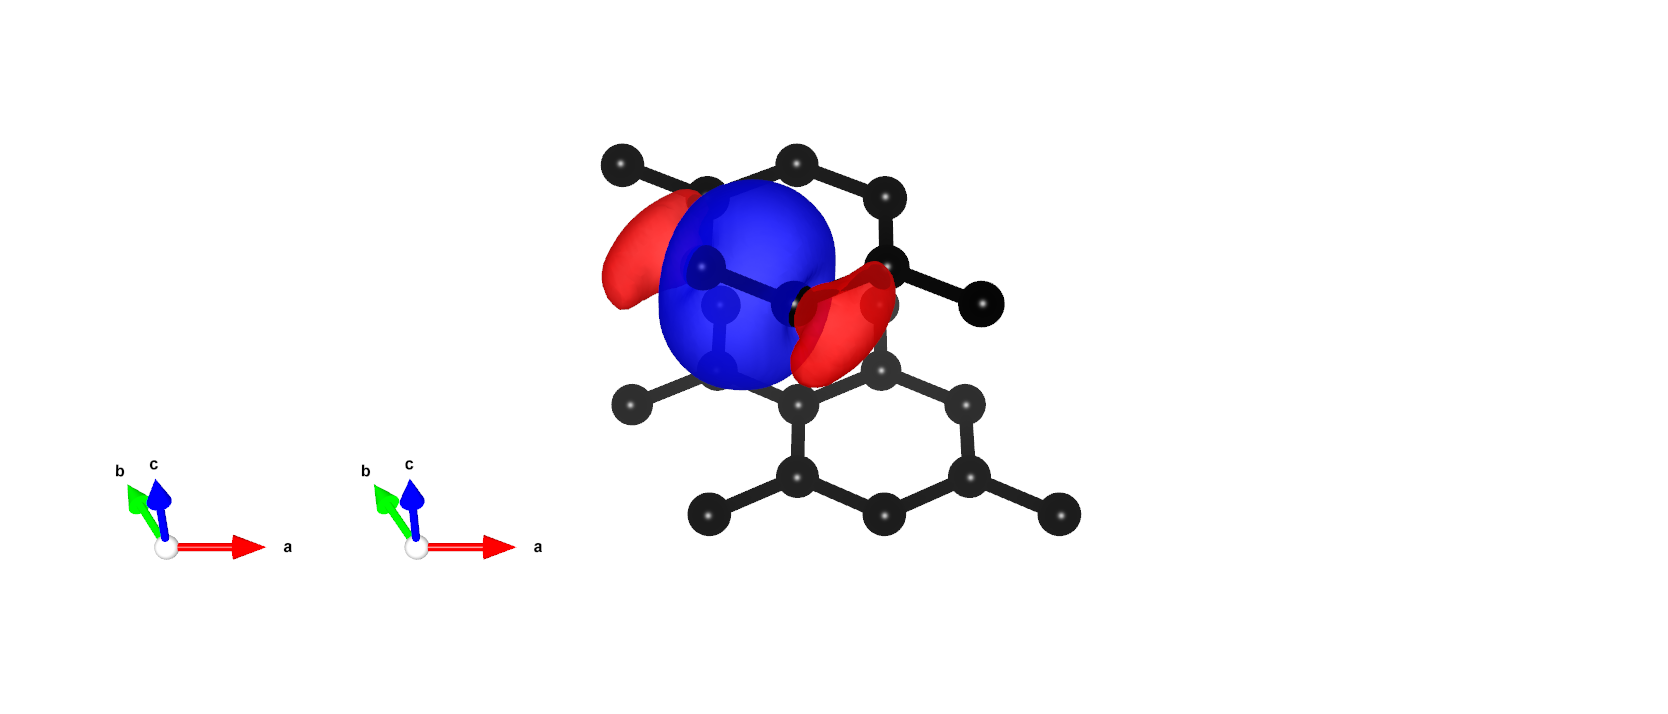
\includegraphics[width=0.3\columnwidth,trim={300pt 100pt 500pt 100pt},clip]{figure/example10/graphite_1.png}}
\centering
\subfloat[$p_z$ top layer]{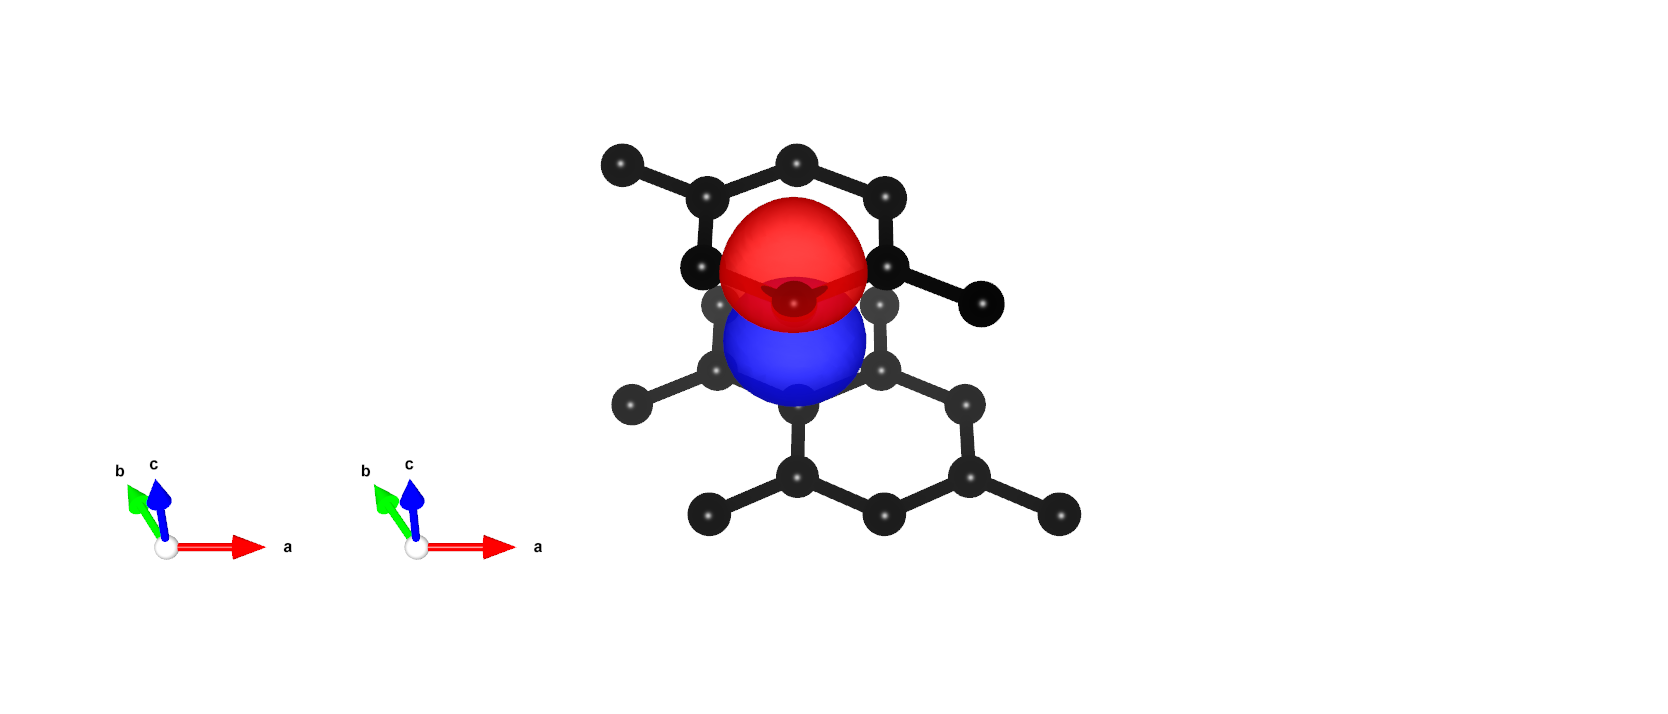
\includegraphics[width=0.3\columnwidth,trim={300pt 100pt 500pt 100pt},clip]{figure/example10/graphite_4.png}}
\centering
\subfloat[$p_z$ bottom layer]{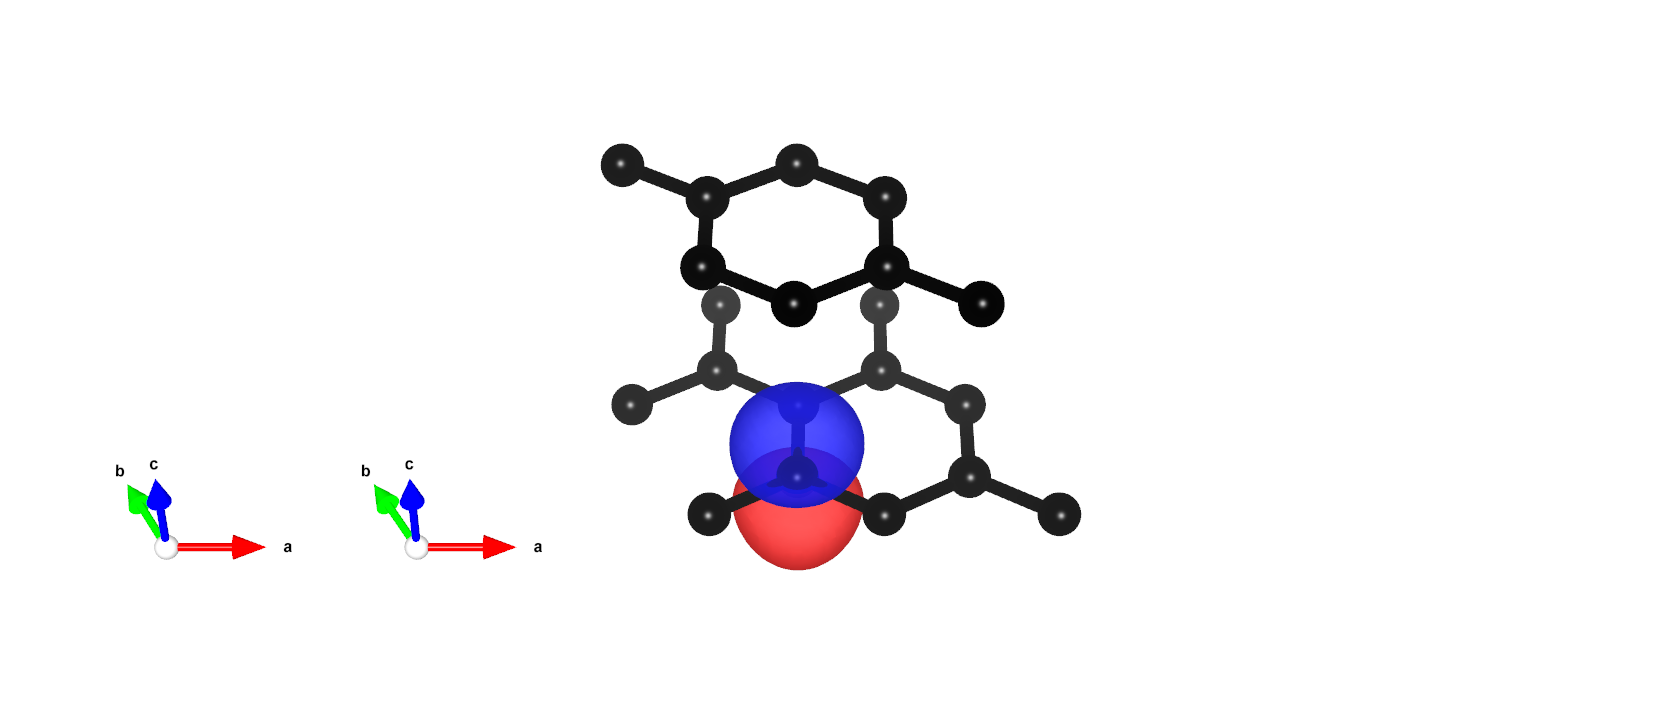
\includegraphics[width=0.3\columnwidth,trim={300pt 100pt 500pt 100pt},clip]{figure/example10/graphite_9.png}}
\caption{MLWFs for graphite. (a) $\sigma$--like MLWF centred on a C--C bond. (b) $p_z$--like MLWF on the top layer. (c) $p_z$--like MLWF on the bottom layer.}\label{fig10.1}
\end{figure}


\begin{table}[h!]
	\centering
	\captionsetup{width=.5\textwidth}
	\caption{Converged values of the components of spread functional and their sums for graphite (AB, Bernal) in \angsqd{}.}
	\begin{tabular}{@{} lllll @{}}\toprule[1.5pt]
	$\Omega$ & $\Omega\tinysub{I}$ & $\Omega\tinysub{OD}$ & $\Omega\tinysub{D}$ & $N_{\mathrm{iter}}$ \\\midrule
	7.3809 & 5.7641 & 1.5874 & 0.0293 & 100 \\\bottomrule[1pt]
	\end{tabular}\label{tab10.1}
\end{table} 
